\documentclass[a4paper,twoside,11pt]{article}
\usepackage[utf8]{inputenc}
\usepackage[english]{babel}
\usepackage{graphicx}
\usepackage{url}
\usepackage{hyperref}
\usepackage{adjustbox}

% pdflatex

% redefinição das margens das páginas
\setlength{\textheight}{24.00cm}
\setlength{\textwidth}{15.50cm}
\setlength{\topmargin}{0.35cm}
\setlength{\headheight}{0cm}
\setlength{\headsep}{0cm}
\setlength{\oddsidemargin}{0.25cm}
\setlength{\evensidemargin}{0.25cm}

\begin{document}

\begin{titlepage}
\begin{center}

% Logo
\resizebox{80mm}{!}{
\includegraphics{../img/logoISEL}}

\vspace{1cm}

% Title
{\Large \textbf{Project and Seminar}\\}
\vspace{0.3cm}
{\Large 2024/2025 - 2nd Semester\\}
\vspace{0.8cm}
{\Large Bachelor in Computer Engineering and Informatics\\}
\vspace{1cm}
{\Huge \textbf{Database Documentation}\\}
\vspace{2cm}

% Authors
\begin{tabular}{c}
    Ângelo Azevedo, n.º 50565, e-mail: \href{mailto:a50565@alunos.isel.pt}{a50565@alunos.isel.pt}\\
    António Alves, n.º 50539, e-mail: \href{mailto:a50539@alunos.isel.pt}{a50539@alunos.isel.pt}\\
\end{tabular}

\vspace{2cm}

% Supervisors
\begin{tabular}{ll}
    {Advisor:} & Pedro Matutino, e-mail: \href{mailto:pedro.miguens@isel.pt}{pedro.miguens@isel.pt} \\
\end{tabular}

\vspace{1cm}

March 2025

\end{center}
\end{titlepage}

\section{Introduction}
This document provides a comprehensive overview of the database structure, including its entities, attributes, and relationships. 
It also details key implementation decisions.

\section{Database overview}
The database has been designed using an Entity-Relationship (ER) approach.
This methodology enables a clear understanding of how different entities interact within the system. The following section presents the ER model diagram.

The database is implemented using PostgreSQL and has been tested with sample data in a Docker container.

The next section will present the ER model in detail.
\section{Entity-Relationship Model}
\begin{figure}[htbp]
	\centering
	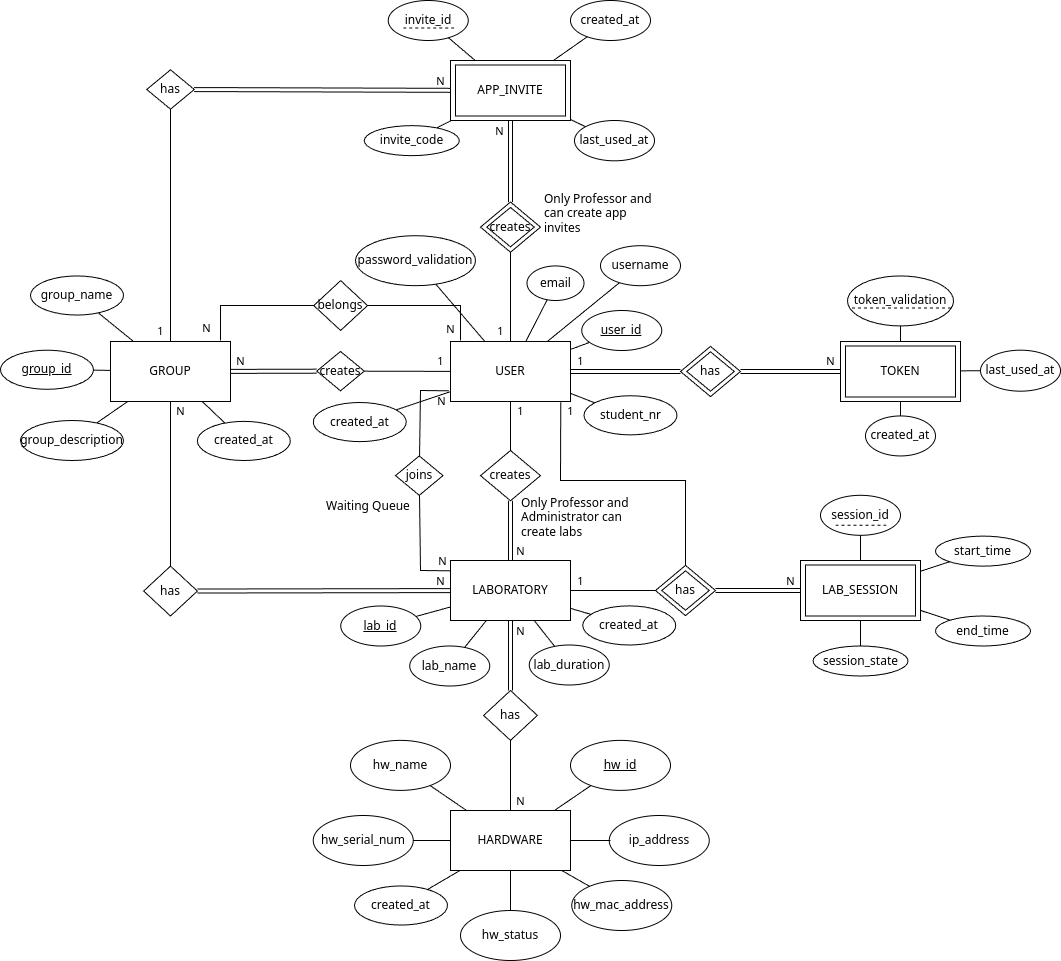
\includegraphics[width=\textwidth]{../img/ERDiagramRL.drawio}
	\caption{Entity-Relationship Model}
	\label{fig:ERModel}
\end{figure}

\section{Entities and Attributes}
This section provides a comprehensive description of each entity and their attributes.
\subsection{User}
The \textbf{User} is a fundamental entity in the database that represents system users.

It has a \textbf{user\_id} as its primary key, implemented as an identity column. An identity column automatically generates values from an implicit sequence.
Therefore, whenever a new user is created, a unique id is automatically generated. The user\_id is an integer data type, chosen to simplify database queries by using a simple numeric identifier instead of email or username.

The entity includes character sequence attributes: \textbf{password\_validation}, \textbf{username} and \textbf{email}. All these fields are required (not null), and the email must be unique. The password\_validation attribute stores a hash of the user's password.
Initially, the username is automatically set to match the user's email during account creation. Users can later modify their username to a preferred value. While usernames are used for display purposes and may not be unique, emails serve as unique identifiers for user searches. The specific constraints for these attributes are defined in the application domain.

Additionally, it includes a \textbf{student\_nr} (student number) as a unique integer field and \textbf{created\_at} as a required timestamp.
The student number is optional, allowing the system to accommodate non-student users such as professors. Notably, there is no discriminator attribute as user type distinctions are handled through the Role-Based Access Control (RBAC) system.

\subsection{Token}
\textbf{Token} is implemented as a weak entity since it cannot exist independently and requires a user\_id for identification. Each token is associated with a user and is essential for authentication purposes. Users must have a valid token when interacting with the system.

As a weak entity, it requires a partial key, which is the \textbf{token\_validation} field. This attribute stores a randomly generated hash created by the system and is used to verify token validity. 
For instance, when a user's token is included in an authorization header, the system compares it with this stored value during each interaction. It is implemented as a required character sequence.

The entity also includes \textbf{created\_at} and \textbf{last\_used\_at} timestamps, both required fields. These attributes enable token validity checking based on timing rules defined by the application domain.

\subsection{App Invite}
\textbf{App Invite} is implemented as a weak entity that depends on the User entity for its existence. Like tokens, app invites cannot exist without an associated user and are automatically removed if the user is deleted. App invites are required for new user registration in the system.

The entity's partial key consists of \textbf{invite\_id} combined with user\_id. The invite\_id is an auto-generated integer identity column, which simplifies invite identification and querying when used in conjunction with the user\_id.

It includes an \textbf{invite\_code} attribute as a required character sequence. While the field can store up to 255 bytes, the actual length restriction is determined by the application domain. This generous byte allocation allows for potential future expansion of the invite code length.

Similar to the Token entity, it includes \textbf{created\_at} and \textbf{last\_used\_at} timestamp fields. These attributes help track invite expiration and can provide valuable usage statistics.

\subsection{Group}
The \textbf{Group} entity represents various types of user groupings, such as student classes, work groups, or professor groups.

Each group has a \textbf{group\_id} as its primary key, implemented as an auto-generated integer identity column. This unique identifier facilitates efficient querying and group identification.

The \textbf{group\_name} is a required character sequence that stores the user-defined name for the group. Group names can be modified after creation, with specific length and format restrictions defined by the application domain.

Groups can include an optional \textbf{group\_description} stored as a text type. This field allows users to provide detailed information about the group's purpose or characteristics. While technically unlimited in length, practical limitations may be imposed by the application domain.

The entity also includes a \textbf{created\_at} timestamp, which can be used for analytical and administrative purposes.

\subsection{Laboratory}
The \textbf{Laboratory} entity represents physical or virtual laboratory spaces within the system.

Each laboratory has a \textbf{lab\_id} as its primary key, implemented as an auto-generated integer identity column. This unique identifier simplifies laboratory identification and database queries.

The \textbf{lab\_name} attribute is a required character sequence that stores the laboratory's designation. Specific naming conventions and restrictions are defined by the application domain.

The entity includes a \textbf{lab\_duration} attribute, which specifies the standard duration of laboratory sessions in minutes. This integer field is required and helps manage session scheduling.

Additionally, it includes a \textbf{created\_at} timestamp for tracking laboratory creation and administrative purposes.

\subsection{Lab Session}
\textbf{Lab Session} is implemented as a weak entity that depends on both User and Laboratory entities. A session represents a specific time period during which a user can access and operate laboratory equipment.

The entity uses \textbf{session\_id} as a partial key, which, combined with user\_id and lab\_id, uniquely identifies each session. The session\_id is an auto-generated integer identity column that facilitates session tracking and queries.

Each session includes required \textbf{start\_time} and \textbf{end\_time} timestamps that define the session's temporal boundaries.

The \textbf{state} attribute is a required character sequence that indicates the session's current status (e.g., active, inactive, or scheduled). The system can be extended to support additional states as needed, with any such changes to be documented in future updates.

\subsection{Hardware}
The \textbf{Hardware} entity represents physical equipment within the laboratory system, such as computers or FPGAs.

Each piece of hardware is identified by a \textbf{hw\_id} primary key, implemented as an auto-generated integer identity column to facilitate equipment tracking and queries.

The entity includes a required \textbf{hw\_name} attribute as a character sequence for equipment identification.

A required \textbf{hw\_serial\_num} character sequence stores the hardware's serial number for inventory management.

The \textbf{ip\_address} and \textbf{hw\_mac\_address} are character sequence fields that may be null depending on the hardware type, as not all equipment requires network connectivity.

A required \textbf{hw\_status} character sequence tracks the current state of the hardware (e.g., available, occupied).

Like other entities, it includes a \textbf{created\_at} timestamp for inventory tracking and administrative purposes.

\section{Associations}
This section details the relationships between entities, explaining how they interact within the system and what restrictions they have.

\textbf{User} associations include:
\begin{itemize}
    \item \textbf{Token} - A weak association where each user may have multiple tokens (N:1). Tokens are automatically generated by the system as needed, with the user's primary key serving as part of the token's composite key.
    \item \textbf{App Invite} - A weak association where users can create multiple app invites (N:1). The user's primary key is incorporated into the app invite's key structure. Only a user with Professor's role can create app invites. 
    It is worth noting that an Administrator can also hold the position of Professor due to hierarchical considerations.    \item \textbf{Group} - Users have two distinct relationships with groups:
    \begin{itemize}
        \item \textbf{creates} - Users can create multiple groups, but each group has exactly one creator (N:1). Only Professor can create groups.
        \item \textbf{belongs} - Users can belong to multiple groups, and groups can have multiple members (N:N)
    \end{itemize}
    \item \textbf{Laboratory} - Users have two types of laboratory associations:
    \begin{itemize}
        \item \textbf{creates} - Users can create multiple laboratories, but each laboratory has one creator (N:1). Only Professor can create laboratories.
        \item \textbf{joins} - Users can join multiple laboratories over time, and laboratories can be joined by multiple users (N:N). While the application domain may impose restrictions (e.g., limiting concurrent laboratory access), the database structure maintains this flexibility to support historical tracking.
    \end{itemize}
    \item \textbf{Lab Session} - A weak association where users can have multiple sessions, but each session belongs to exactly one user (N:1)
\end{itemize}

\textbf{App Invite} maintains an additional association with the Group entity, linking invites to specific groups. Each invite corresponds to one group, while groups can have multiple associated invites (N:1). This enables automatic group assignment upon registration.

\textbf{Group} has an additional association with Laboratory, controlling laboratory access permissions. Groups can be associated with multiple laboratories, and laboratories can be accessible to multiple groups (N:N).

\textbf{Laboratory} maintains these additional associations:
\begin{itemize}
    \item \textbf{Lab Session} - Laboratories can have multiple sessions, but each session is associated with exactly one laboratory (N:1)
    \item \textbf{Hardware} - Laboratories can be assigned multiple pieces of hardware, and hardware can be assigned to multiple laboratories over time (N:N)
\end{itemize}

Note that additional constraints and business rules are implemented at the web API level. Please refer to the web API documentation for detailed information about these restrictions.


\renewcommand{\refname}{\section{Bibliography}}
\begin{thebibliography}{1}
\bibitem{postgresql} PostgreSQL Global Development Group. \textit{PostgreSQL Documentation}. [Online]. Available: \url{https://www.postgresql.org/docs/}
\end{thebibliography}

\end{document}